\section{条件期望的不等式}
\label{sec:cexp-inequalities}

条件期望对线性运算可以逐项进行，对非线性运算却不行：$\mathbb{E}[Y^{2}\mid X]$与$(\mathbb{E}[Y\mid X])^{2}$一般不相等。传感器表的第二行中，前者是$3/2$，后者是$1$。“先在组内平均再平方”与“先平方再在组内平均”之间的差别有确定的方向吗？第~\ref{chap:random-variable-moments}章用凸函数回答了不带条件的情形，这一节把它推广到给定信息的情形，再把绝对值的幂作为特例，得到条件期望对$L^{p}$大小的控制。

\subsection{条件Jensen不等式}
\label{sec:cexp-jensen}

\paragraph{可数条支撑线}
第~\ref{chap:random-variable-moments}章的Jensen不等式在$\mathbb{E}[X]$这一点放一条支撑线，再对两边取期望。给定信息时，条件平均$\mathbb{E}[X\mid\mathcal{G}]$随样本点变化，支撑点也随之变化，需要同时用到许多条支撑线。每条支撑线给出的不等式都只在一个零概率集之外成立，为了能把例外集并起来，支撑线只能取可数多条。下面的引理说明可数条已经足够。

\begin{lemma}[凸函数是可数条直线的上包络]
\label{lem:cexp-countable-lines}
设$\varphi:\mathbb{R}\to\mathbb{R}$是凸函数。对每个有理数$q$，取$\varphi$在$q$处的一条支撑线的斜率$s_q$，即$\varphi(x)\geq\varphi(q)+s_q(x-q)$对一切$x$成立。则对每个实数$x$，
\begin{equation}
 \varphi(x)=\sup_{q\in\mathbb{Q}}\bigl(\varphi(q)+s_q(x-q)\bigr).
 \label{eq:cexp-countable-lines}
\end{equation}
\end{lemma}

\begin{proof}
支撑线的存在见第~\ref{chap:random-variable-moments}章。由支撑线的定义，右边不超过$\varphi(x)$，只需说明右边能任意接近$\varphi(x)$。

先说明靠近$x$的支撑点上，斜率有统一的界。凸函数在$\mathbb{R}$上连续，设$\lvert\varphi\rvert$在$[x-2,x+2]$上不超过$M$。对$q\in[x-1,x+1]$，把支撑线不等式用在$x+2$处，移项得
\[
 s_q\leq\frac{\varphi(x+2)-\varphi(q)}{x+2-q}\leq\frac{2M}{1}=2M ,
\]
这里用了$x+2-q\geq1$。同样把它用在$x-2$处，得$s_q\geq-2M$。所以$\lvert s_q\rvert\leq2M$。

于是对$q\in[x-1,x+1]\cap\mathbb{Q}$，
\[
 \varphi(q)+s_q(x-q)\geq\varphi(q)-2M\lvert x-q\rvert .
\]
令有理数$q\to x$，由$\varphi$的连续性，右边趋于$\varphi(x)$。
\end{proof}

\paragraph{不等式与证明}
有了可数条支撑线，对每一条用一次条件期望的线性与保序，再取上确界。

\begin{theorem}[条件Jensen不等式]
\label{thm:cexp-jensen}
设$\varphi:\mathbb{R}\to\mathbb{R}$是凸函数，$X$与$\varphi(X)$都可积。则
\begin{equation}
 \varphi\bigl(\mathbb{E}[X\mid\mathcal{G}]\bigr)\leq\mathbb{E}\bigl[\varphi(X)\bigm|\mathcal{G}\bigr].
 \label{eq:cexp-jensen}
\end{equation}
\end{theorem}

\begin{proof}
记$Z=\mathbb{E}[X\mid\mathcal{G}]$。对每个有理数$q$，由支撑线不等式，
\[
 \varphi(X)\geq\varphi(q)+s_q(X-q)
\]
处处成立。两边都可积，由定理~\ref{thm:cexp-linearity}的保序与线性，存在零概率事件$N_q$，在$N_q$之外
\[
 \mathbb{E}\bigl[\varphi(X)\bigm|\mathcal{G}\bigr]\geq\varphi(q)+s_q(Z-q).
\]
令$N=\bigcup_{q\in\mathbb{Q}}N_q$，它是可数个零概率事件之并，概率仍为零。在$N$之外，上式对所有有理数$q$同时成立，对$q$取上确界，由式~\eqref{eq:cexp-countable-lines}，右边成为$\varphi(Z)$。
\end{proof}

式~\eqref{eq:cexp-jensen}称为\term{条件Jensen不等式}（conditional Jensen inequality）。定理的条件各有作用。凸性决定方向：组内平均把点拉向组内的重心，凸函数在重心处的值不超过函数值的平均。$X$与$\varphi(X)$可积，保证两边的条件期望都有定义。可数性藏在证明里：如果直接对每个实数$q$使用支撑线，会得到不可数多个例外集，它们的并可能不是零概率集。

\paragraph{用平方函数检验方向}
取$\varphi(y)=y^{2}$。设$X$平方可积，式~\eqref{eq:cexp-jensen}给出
\[
 \bigl(\mathbb{E}[X\mid\mathcal{G}]\bigr)^{2}\leq\mathbb{E}[X^{2}\mid\mathcal{G}] .
\]
传感器表三行的两边依次是
\[
 \tfrac19\leq\tfrac13,\qquad 1\leq\tfrac32,\qquad \tfrac{25}{9}\leq3 ,
\]
差值$2/9$、$1/2$、$2/9$正是第~\ref{chap:random-vectors}章算出的三行条件方差，第~\ref{sec:cexp-conditional-variance}节会在一般情形下定义它。图~\ref{fig:cexp-jensen}(a)画出第二行的几何：三个点$(y,y^{2})$按条件概率$\tfrac14,\tfrac12,\tfrac14$加权，重心的高度是$3/2$，高于抛物线在重心横坐标$1$处的高度$1$；紫色虚线是$y=1$处的支撑线。

\begin{BookInlineFigure}
  \centering
  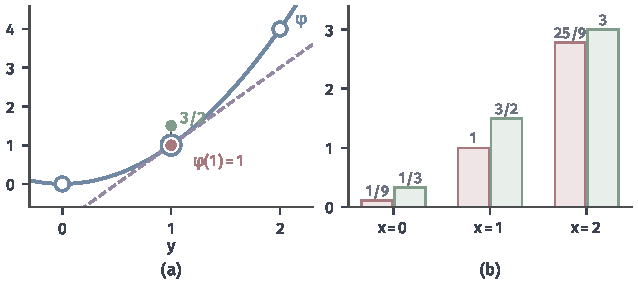
\includegraphics[width=108mm]{figures/07-probability/02-measure-theoretic-probability/matplotlib/cexp-jensen/figure.pdf}
  \caption{条件Jensen不等式，$\varphi(y)=y^{2}$，传感器表。(a)第二行$X=1$：空心圆是$(y,y^{2})$，大小与条件概率$\tfrac14,\tfrac12,\tfrac14$成正比；红点是$\varphi(\mathbb{E}[Y\mid X=1])=1$，绿点是$\mathbb{E}[Y^{2}\mid X=1]=3/2$，紫色虚线是$y=1$处的支撑线。(b)三行的$(\mathbb{E}[Y\mid X=x])^{2}$（红）与$\mathbb{E}[Y^{2}\mid X=x]$（绿）。}
  \label{fig:cexp-jensen}
\end{BookInlineFigure}

若$\varphi$是凹函数，对$-\varphi$用定理，不等号反向。例如对凹函数$-y^{2}$，得到的不等式两边乘以$-1$后就是上面的平方不等式。既不凸也不凹的函数没有确定的方向。取$\varphi(y)=y^{3}$，它在$[0,\infty)$上凸，在$(-\infty,0]$上凹。传感器表第一行中$Y$以$\tfrac23,\tfrac13$取$0,1$，两个值落在凸段上，
\[
 \bigl(\mathbb{E}[Y\mid X=0]\bigr)^{3}=\tfrac{1}{27}<\tfrac13=\mathbb{E}[Y^{3}\mid X=0].
\]
把变量平移成$Y-2$，第一行的两个值$-2,-1$落在凹段上，方向随之反转：
\[
 \bigl(\mathbb{E}[Y-2\mid X=0]\bigr)^{3}=-\tfrac{125}{27}\approx-4.63>-\tfrac{17}{3}\approx-5.67=\mathbb{E}\bigl[(Y-2)^{3}\bigm|X=0\bigr].
\]
同一个函数，作用在落于不同区段的取值上，可以给出相反的方向；只有在整个$\mathbb{R}$上凸，才能对一切变量和一切信息保证式~\eqref{eq:cexp-jensen}。

\subsection{\texorpdfstring{$L^p$}{Lp}收缩}
\label{sec:cexp-lp}

\paragraph{条件平均不放大\texorpdfstring{$L^{p}$}{Lp}范数}
对$1\leq p<\infty$，记
\[
 \lVert X\rVert_p=\bigl(\mathbb{E}\lvert X\rvert^{p}\bigr)^{1/p},
\]
$L^{p}$是满足$\lVert X\rVert_p<\infty$的随机变量组成的空间，两个几乎必然相等的随机变量视为同一个元素，见\BookChapterRef{chap:function-normed-spaces}{卷四第11章“赋范空间”}。在概率空间上，$L^{p}\subseteq L^{1}$：由逐点的不等式$\lvert x\rvert\leq1+\lvert x\rvert^{p}$取期望，得到$X$可积。再对凸函数$y\mapsto\lvert y\rvert^{p}$和可积的$\lvert X\rvert$用第~\ref{chap:random-variable-moments}章的Jensen不等式，
\[
 \bigl(\mathbb{E}\lvert X\rvert\bigr)^{p}\leq\mathbb{E}\lvert X\rvert^{p},
\]
即$\lVert X\rVert_1\leq\lVert X\rVert_p$。所以$L^{p}$中的随机变量都有条件期望。把条件Jensen不等式用于$\varphi(y)=\lvert y\rvert^{p}$，就得到条件期望对$L^{p}$范数的控制。

\begin{theorem}[\texorpdfstring{$L^{p}$}{Lp}收缩]
\label{thm:cexp-lp}
设$1\leq p<\infty$，$X\in L^{p}$。则$\mathbb{E}[X\mid\mathcal{G}]\in L^{p}$，并且
\begin{equation}
 \bigl\lVert\mathbb{E}[X\mid\mathcal{G}]\bigr\rVert_p\leq\lVert X\rVert_p .
 \label{eq:cexp-lp}
\end{equation}
\end{theorem}

\begin{proof}
$\varphi(y)=\lvert y\rvert^{p}$是$\mathbb{R}$上的凸函数，$X$与$\lvert X\rvert^{p}$都可积。由条件Jensen不等式，
\[
 \bigl\lvert\mathbb{E}[X\mid\mathcal{G}]\bigr\rvert^{p}\leq\mathbb{E}\bigl[\lvert X\rvert^{p}\bigm|\mathcal{G}\bigr].
\]
两边非负，取期望，右边由全期望公式等于$\mathbb{E}\lvert X\rvert^{p}$，于是
\[
 \mathbb{E}\bigl\lvert\mathbb{E}[X\mid\mathcal{G}]\bigr\rvert^{p}\leq\mathbb{E}\lvert X\rvert^{p}<\infty .
\]
两边开$p$次方即得。
\end{proof}

$p=\infty$的情形更直接：若$\lvert X\rvert\leq c$几乎必然成立，由保序，$\lvert\mathbb{E}[X\mid\mathcal{G}]\rvert\leq c$几乎必然成立。

\paragraph{对扰动的稳定性}
把定理用于两个输入之差。设$X_1,X_2\in L^{p}$，由线性，
\begin{equation}
 \bigl\lVert\mathbb{E}[X_1\mid\mathcal{G}]-\mathbb{E}[X_2\mid\mathcal{G}]\bigr\rVert_p\leq\lVert X_1-X_2\rVert_p .
 \label{eq:cexp-lp-stability}
\end{equation}
条件期望是$L^{p}$上的线性映射，范数不超过$1$：输入有一点扰动，输出的扰动不会更大。由此，若$X_n\to X$在$L^{p}$中成立，则$X_n$的条件期望也在$L^{p}$中收敛到$\mathbb{E}[X\mid\mathcal{G}]$，条件期望与$L^{p}$极限可以交换次序。

\paragraph{逐次等分的数值}
用逐次等分的例子观察这个不等式，把$X$中心化，取$X(\omega)=\omega^{2}-\tfrac13$。$n=1$时，两段上的平均是$\tfrac1{12}-\tfrac13$与$\tfrac{7}{12}-\tfrac13$，即
\[
 \mathbb{E}[X\mid\mathcal{G}_1]=-\tfrac14\ \text{在}\ [0,\tfrac12)\ \text{上},\qquad
 \mathbb{E}[X\mid\mathcal{G}_1]=\tfrac14\ \text{在}\ [\tfrac12,1)\ \text{上}.
\]
$\lvert\mathbb{E}[X\mid\mathcal{G}_1]\rvert$恒为$1/4$，所以它的各阶范数都是$1/4$。另一方面，$X$在$\omega_0=1/\sqrt3$处变号，分两段积分，
\[
 \lVert X\rVert_1=\int_0^{\omega_0}\Bigl(\frac13-\omega^{2}\Bigr)\mathrm{d}\omega+\int_{\omega_0}^{1}\Bigl(\omega^{2}-\frac13\Bigr)\mathrm{d}\omega=\frac{4}{9\sqrt3}\approx0.2566 .
\]
$\lVert X\rVert_2^{2}$是$\omega^{2}$的方差$\tfrac15-\tfrac19=\tfrac4{45}$，所以$\lVert X\rVert_2\approx0.2981$。两者都大于$1/4$，与式~\eqref{eq:cexp-lp}一致。

图~\ref{fig:cexp-lp-contraction}(a)画出$n=0,1,\dots,7$时$\lVert\mathbb{E}[X\mid\mathcal{G}_n]\rVert_p$，三条绿色折线分别对应$p=1,2,4$，都停在紫色虚线$\lVert X\rVert_p$之下。折线随$n$不减，这可以由塔式法则解释：$\mathcal{G}_n\subseteq\mathcal{G}_{n+1}$，由式~\eqref{eq:cexp-tower}，
\[
 \mathbb{E}[X\mid\mathcal{G}_n]=\mathbb{E}\bigl[\mathbb{E}[X\mid\mathcal{G}_{n+1}]\bigm|\mathcal{G}_n\bigr],
\]
把$\mathbb{E}[X\mid\mathcal{G}_{n+1}]$当作输入，对右边用式~\eqref{eq:cexp-lp}，得到
\[
 \bigl\lVert\mathbb{E}[X\mid\mathcal{G}_n]\bigr\rVert_p\leq\bigl\lVert\mathbb{E}[X\mid\mathcal{G}_{n+1}]\bigr\rVert_p .
\]
图中各折线还逐渐贴近上界。信息逐步增加时条件期望的收敛属于鞅的理论，可参考\BookChapterRef{chap:discrete-time-stochastic-processes}{卷九第3章“离散时间随机过程”}；这里只把它作为数值观察。

\begin{BookInlineFigure}
  \centering
  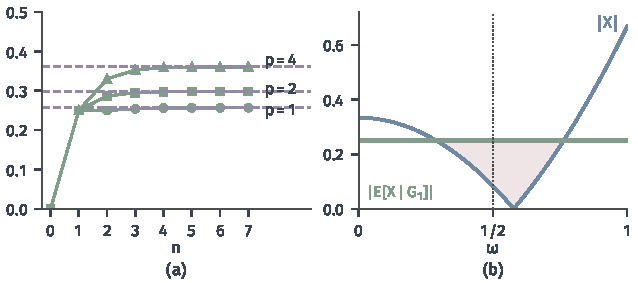
\includegraphics[width=108mm]{figures/07-probability/02-measure-theoretic-probability/matplotlib/cexp-lp-contraction/figure.pdf}
  \caption{$L^{p}$收缩，$\Omega=[0,1)$，$X(\omega)=\omega^{2}-\tfrac13$，$\mathcal{G}_n$由$2^{n}$个等长区间生成，范数用$2^{16}$个小区间上的中点公式计算。(a)$\lVert\mathbb{E}[X\mid\mathcal{G}_n]\rVert_p$（绿；圆、方、三角分别对应$p=1,2,4$）与$\lVert X\rVert_p$（紫色虚线）。(b)$n=1$时的$\lvert X\rvert$（蓝）与$\lvert\mathbb{E}[X\mid\mathcal{G}_1]\rvert$（绿），浅红区域上后者更大。}
  \label{fig:cexp-lp-contraction}
\end{BookInlineFigure}

\paragraph{控制的是总体大小}
式~\eqref{eq:cexp-lp}控制的是范数，即对整个$\Omega$平均后的大小，不是逐点的大小。图~\ref{fig:cexp-lp-contraction}(b)中，$\omega$在$\omega_0\approx0.577$附近时$\lvert X\rvert$接近$0$，而$\lvert\mathbb{E}[X\mid\mathcal{G}_1]\rvert=1/4$，浅红区域上条件平均的绝对值比原变量大。组内平均把组内的值拉向同一个数，原来接近零的样本点被拉离零，原来远离零的被拉近；拉近的部分在范数中占上风。传感器表中同样如此：格子$(0,0)$上$Y=0$，$\mathbb{E}[Y\mid X]=1/3$。
